\documentclass[a4paper,14pt]{extarticle}

\newcommand{\stend}{\textbf{Wb-demo-kit v.2}}

% Путь до папки с общими шаблонами
\newcommand{\pathToCommonFolder}{/home/denilai/Documents/repos/latex/Common}

% Название работы в титуле
\newcommand{\workname}{Отчет по практической работе №3}
% Название дисциплины в титуле
\newcommand{\discipline}{Проектирование информационных систем}
% Название кафедры в титуле
\newcommand{\kafedra}{Кафедра инструментального и прикладного программного обеспечения}
% Тема работы в титуле
\newcommand{\theme}{Функциональное проектирование модели информационной системы с использованием методологии SADT}
% Должность преподавателя в титуле
\newcommand{\rang}{ассистент}

% ФИО студента в титуле
\newcommand{\studentfio}{К.~Ю.~Денисов}%\\Д.~Н.~Федосеев\\А.~М.~Сосунов}\\%К.~Ю.~Денисов\\%И.~А.~Кремнев
% ФИО преподавателя в титуле
\newcommand{\teacherfio}{А.~А.~Русляков}


\usepackage{tabularx}
\usepackage{lastpage}


\usepackage{booktabs}
\newcolumntype{b}{X}
\newcolumntype{s}{>{\hsize=.5\hsize}X}
\newcommand{\heading}[1]{\multicolumn{1}{c}{#1}}

% установка размера шрифта для всего документа
%\fontsize{20pt}{18pt}\selectfont
\usepackage{extsizes} % Возможность сделать 14-й шрифт

% Вставка заготовки преамбулы
% Этот шаблон документа разработан в 2014 году
% Данилом Фёдоровых (danil@fedorovykh.ru) 
% для использования в курсе 
% <<Документы и презентации в \LaTeX>>, записанном НИУ ВШЭ
% для Coursera.org: http://coursera.org/course/latex .
% Исходная версия шаблона --- 
% https://www.writelatex.com/coursera/latex/5.3

% В этом документе преамбула

% Для корректного использования русских символов в формулах
% пакеты hyperref и настройки, связанные с ним, стоит загуржать
% перед загрузкой пакета mathtext



% поддержка русских букв
% кодировка шрифта
%\usepackage[T2A]{fontenc} 
\usepackage{pscyr}

% использование ненумеровонного абзаца с добавлением его в содержаниеl

\newcommand{\anonsection}[1]{\section*{#1}\addcontentsline{toc}{section}{#1}}
\newcommand{\sectionunderl}[1]{\section*{\underline{#1}}}


% настройка окружения enumerate
\usepackage{enumitem}
\setlist{noitemsep}
\setlist[enumerate]{labelsep=*, leftmargin=1.5pc}

\usepackage{hyperref}

% сначала ставить \usepackage{extsizes} % Возможность сделать 14-й шрифт
% для корректной установки полей вставлять преамбулу следует в последнюю очередь (но перед дерективой замены \rmdefault)
\usepackage[top=20mm,bottom=25mm,left=35mm,right=20mm]{geometry} % Простой способ задавать поля

\hypersetup{				% Гиперссылки
	unicode=true,           % русские буквы в раздела PDF
	pdftitle={Заголовок},   % Заголовок
	pdfauthor={Автор},      % Автор
	pdfsubject={Тема},      % Тема
	pdfcreator={Создатель}, % Создатель
	pdfproducer={Производитель}, % Производитель
	pdfkeywords={keyword1} {key2} {key3}, % Ключевые слова
	colorlinks=true,       	% false: ссылки в рамках; true: цветные ссылки
	linkcolor=red,          % внутренние ссылки
	citecolor=black,        % на библиографию
	filecolor=magenta,      % на файлы
	urlcolor=blue           % на URL
}

%%% Работа с русским языком
\usepackage{cmap}					% поиск в PDF
\usepackage{mathtext} 				% русские буквы в формулах
\usepackage[T2A]{fontenc}			% кодировка
\usepackage[utf8]{inputenc}			% кодировка исходного текста
\usepackage[english,russian]{babel}	% локализация и переносы
\usepackage{indentfirst}
\frenchspacing

%для изменения названия списка иллюстраций
\usepackage{tocloft}


\renewcommand{\epsilon}{\ensuremath{\varepsilon}}
\renewcommand{\phi}{\ensuremath{\varphi}}
\renewcommand{\kappa}{\ensuremath{\varkappa}}
\renewcommand{\le}{\ensuremath{\leqslant}}
\renewcommand{\leq}{\ensuremath{\leqslant}}
\renewcommand{\ge}{\ensuremath{\geqslant}}
\renewcommand{\geq}{\ensuremath{\geqslant}}
\renewcommand{\emptyset}{\varnothing}

% Изменения параметров списка иллюстраций
\renewcommand{\cftfigfont}{Рисунок } % добавляем везде "Рисунок" перед номером
\addto\captionsrussian{\renewcommand\listfigurename{Список иллюстративного материала}}

\newcommand{\tm}{\texttrademark\ }
\newcommand{\reg}{\textregistered\ }


%%% Дополнительная работа с математикой
\usepackage{amsmath,amsfonts,amssymb,amsthm,mathtools} % AMS
\usepackage{icomma} % "Умная" запятая: $0,2$ --- число, $0, 2$ --- перечисление

%% Номера формул
%\mathtoolsset{showonlyrefs=true} % Показывать номера только у тех формул, на которые есть \eqref{} в тексте.
%\usepackage{leqno} % Нумереация формул слева

%% Свои команды
\DeclareMathOperator{\sgn}{\mathop{sgn}}

%% Перенос знаков в формулах (по Львовскому)
\newcommand*{\hm}[1]{#1\nobreak\discretionary{}
{\hbox{$\mathsurround=0pt #1$}}{}}


% отступ для первого абзаца главы или параграфа
%\usepackage{indentfirst}

%%% Работа с картинками
\usepackage{graphicx}  % Для вставки рисунков
\graphicspath{{images/}{screnshots/}}  % папки с картинками
\DeclareGraphicsExtensions{.pdf,.png,.jpg}
\setlength\fboxsep{3pt} % Отступ рамки \fbox{} от рисунка
\setlength\fboxrule{1pt} % Толщина линий рамки \fbox{}
\usepackage{wrapfig} % Обтекание рисунков текстом

%%% Работа с таблицами
\usepackage{array,tabularx,tabulary,booktabs} % Дополнительная работа с таблицами
\usepackage{longtable}  % Длинные таблицы
\usepackage{multirow} % Слияние строк в таблице

%%% Теоремы
\theoremstyle{plain} % Это стиль по умолчанию, его можно не переопределять.
\newtheorem{theorem}{Теорема}[section]
\newtheorem{proposition}[theorem]{Утверждение}

\theoremstyle{plain} % Это стиль по умолчанию, его можно не переопределять.
\newtheorem{work}{Практическая работа}[part]


 
 
\theoremstyle{definition} % "Определение"
\newtheorem{corollary}{Следствие}[theorem]
\newtheorem{problem}{Задача}[section]
 
\theoremstyle{remark} % "Примечание"
\newtheorem*{nonum}{Решение}



%%% Программирование
\usepackage{etoolbox} % логические операторы

%%% Страница

%	\usepackage{fancyhdr} % Колонтитулы
% 	\pagestyle{fancy}
%   \renewcommand{\headrulewidth}{0pt}  % Толщина линейки, отчеркивающей верхний колонтитул
% 	\lfoot{Нижний левый}
% 	\rfoot{Нижний правый}
% 	\rhead{Верхний правый}
% 	\chead{Верхний в центре}
% 	\lhead{Верхний левый}
%	\cfoot{Нижний в центре} % По умолчанию здесь номер страницы

\usepackage{setspace} % Интерлиньяж
\onehalfspacing % Интерлиньяж 1.5
%\doublespacing % Интерлиньяж 2
%\singlespacing % Интерлиньяж 1

\usepackage{lastpage} % Узнать, сколько всего страниц в документе.

\usepackage{soul} % Модификаторы начертания


\usepackage[usenames,dvipsnames,svgnames,table,rgb]{xcolor}


\usepackage{csquotes} % Еще инструменты для ссылок

%\usepackage[style=authoryear,maxcitenames=2,backend=biber,sorting=nty]{biblatex}

\usepackage{multicol} % Несколько колонок

\usepackage{tikz} % Работа с графикой
\usepackage{pgfplots}
\usepackage{pgfplotstable}

% модуль для вставки рыбы
\usepackage{blindtext}

\usepackage{listings}
\usepackage{color}


% для поворота отдельной страницы. Использовать окружение \landscape
\usepackage{pdflscape} 
\usepackage{rotating} 


\definecolor{mygreen}{rgb}{0,0.6,0}
\definecolor{mygray}{rgb}{0.5,0.5,0.5}
\definecolor{mymauve}{rgb}{0.58,0,0.82}


% пример импорта файла
%\lstinputlisting{/home/denilai/repomy/conf/distributions}

\lstset{
	language=Python,
	basicstyle=\footnotesize,        % the size of the fonts that are used for the code
	numbers=left,                    % where to put the line-numbers; possible values are (none, left, right)
	numbersep=5pt,                   % how far the line-numbers are from the code
	numberstyle=\tiny\color{mygray}, % the style that is used for the line-numbers
	stepnumber=2,                    % the step between two line-numbers. If it's 1, each line will be numbered
	% Tab - 2 пробела
	tabsize=2,    
	% Автоматический перенос строк
	breaklines=true,
	frame=single,
	breakatwhitespace=true,
	title=\lstname 
}



\author{Кирилл Денисов}
\title{Лабораторная работа №1}
\date{\today}

\setcounter{withouttheme}{0}
\setcounter{withoutsubmissiondate}{1}

%если нужна тема работы в отчете, то указать в скобках что-либо, иначе оаставить пустым
%\renewcommand{\withouttheme}{}
%если нужна дата представления отчета, то указать в скобках что-либо
%\renewcommand{\withoutsubmissiondate}{1}

% установка полуторного интервала
% \usepackage{setspace}  
% \onehalfspacing

% использовать Times New Roman
\renewcommand{\rmdefault}{ftm}


\newcommand{\tb}{ThingsBoard~}

\begin{document}
	\thispagestyle{empty}
	% Вставка первого титульного листа
	% Есть две версии титульного листа - одиночный (titul) и групповой (titulAll)
	%\newcounter{withouttheme}

%\setcounter{withouttheme}{<n>} установить значение счетчика  withouttheme для определения, нужна ли тема
%    {0} - нужна
%    {1} - не нужна

%\setcounter{withoutsubmissiondate}{<n>} установить значение счетчика  withoutsubmissiondate для определения, нужна ли дата представления к защите
%     {0} - нужна
%     {1} - не нужена
\begin{center}
	\begin{figure}[h!]
		\begin{center}
		%\vspace{-10ex}
		
\includegraphics[width=0.17\linewidth]{\pathToCommonFolder/gerb}
		%\caption{}\label{pic:first}
		%	\vspace{5ex}
		\end{center}	
	\end{figure}
 	\small	МИНОБРНАУКИ РОССИИ \\
	Федеральное государственное бюджетное образовательное учреждение\\
						высшего образования\\
\normalsize					
\textbf{«МИРЭА – Российский технологический университет»\\
						РТУ МИРЭА}\\
						\noindent\rule{1\linewidth}{1pt}\\
       Институт информационных технологий\\ %\vspace{2ex}
					\kafedra\\
		\vspace{3ex}
			\large \textbf{\workname}  \\
		%\vspace{1ex}
						по дисциплине\\ «\discipline» \\
		\vspace{3ex}
		\ifnum \value{withouttheme}=0 {
			\textbf{Тема работы:}\\ <<\theme>>
		}
		\else {}
		\fi
\vspace{10ex}
\small
\begin{table}[h!]
\begin{tabular}{lp{0.6\linewidth}l}
	\textbf{Выполнил:} & студент группы ИВБО-02-19 & \\ 
	& & \studentfio \\%Д.~Н.~Федосеев\\%А.~М.~Сосунов\\%К.~Ю.~Денисов\\%И.~А.~Кремнев
	\textbf{Принял:} & \rang & \\
	& & \teacherfio \hfill\\
\end{tabular}
\end{table}
\end{center}
\ifnum \value{withoutsubmissiondate}=0 {
	\begin{flushleft}
		Работа представлена к защите <<\rule{3ex}{1pt}>>\rule{10ex}{1pt} 202\rule{1ex}{1pt} г.\hfill
	\end{flushleft}
\else {}
\fi

\normalsize
\begin{center}	
\vfill
Москва 2022
\end{center}

	\newpage
	%\tableofcontents
	\newpage
	%\listoftables
	
\normalsize

\section{Цель создания системы}
Разрабатываемая информационная система <<Электронный сборник лабораторных работ>> (далее по тексту Система) служит для сбора, хранения и учета письменных работ различного характера, выполненных учащимися средних общеобразовательных, средних специальных и высших учебных заведений. На данной платформе пользователям на безвозмездной основе предоставляется доступ к загруженным документам, топикам и темам форума и медиафайлам. 

Система выполняет функции образовательной платформы. Платформа может быть интегрирована в информационную среду учебных заведений, предоставляя инструменты для учета и хранения работ учащихся. 


\section{Краткое описание}

Пользователь взаимодействует с системой посредством веб-сервиса.  Сайт является удобным
интернет сервисом, представляющим информацию о персональных файлах, перечне загруженных в Систему работ. Веб-интерфейс реализует возможность доступа к форуму для обсуждений. Для комфортного и
круглосуточного доступа, сайт так же адаптирован для мобильных устройств.

Кроме того, платформа позволяет пользователю просматривать файлы, основываясь на большом количестве поисковых фильтров. Сортировка возможна по времени загрузки, наименованию научной дисциплины, виду и популярности работы.


\section{Средства создания ИС}
В качестве средств создания ИС был использован язык программирования PHP и JavaScript. Для хранения метаданных и системных сообщений используется база данных под управлением СУБД PostreSQL. Для хранения пользовательских файлов используется объектное хранилище под управлением NoSQL базы данных Cassandra.

В качестве инструмента веб-аналитики используется Яндек.Метрика. Данных инструмент помогает получать наглядные отчеты, видеозаписи действий посетителей, отслеживать источники трафика и оценивать эффективность онлайн- и офлайн-рекламы.

Система построена в соответствии с подходом Ajax, заключающийся в <<фоновом>> обмене данными браузера с веб-сервером. В результате при обновлении данных веб-страница не перезагружается полностью, и веб-приложения становятся быстрее и удобнее.

Для моделирования проектируемой ИС будет
использоваться нотация IDEF0 программном обеспечении CASE Ramus
Educational edition.

\section{Проектирование контекстной диаграммы функциональной модели	ИС}

Была спроектирована контекстная диаграмма A–0 в нотации IDEF0.
В качестве входа по управлению (стрелка управления) были выбраны
следующие нормативные и правовые документы:

\begin{enumerate}
	\item 152-ФЗ "О пероснальных данных".
	\item 149-ФЗ "Об информации, информационных технологиях и о защите информации".
	\item Политика интернет-сайта.
	\item Пользовательское соглашение.
\end{enumerate}

В качестве входящих информационных потоков, которые подлежат
обработке и преобразованию в процессе работы ИС была указана следующая
информация:
\begin{enumerate}
	\item Персональные данные пользователя
	\item Пользовательские файлы
\end{enumerate}

В качестве механизмов (ресурсов, выполняющих работу) были
выделены:
\begin{enumerate}
\item Подсистема хранения.
\item Подсистема обработки запросов.
\item Подсистема технической поддержки.
\item Подсистема личного кабинета.
\item Подсистема форума.
\item Модератор форума.
\item Пользователь системы.
\end{enumerate}

В качестве выходов после выполнения ИС получены следующие
информационные элементы:
\begin{enumerate}
	\item Статистические данные об активности пользователей.
	\item Сведения о работе подсистем.
\end{enumerate}

Так как механизмы <<Подсистема хранения>>, <<Подсистема обработки запросов>> и <<Пользователь системы>> 
%и входы по управлению <<152-ФЗ 'О пероснальных данных'>> и <<149-ФЗ 'Об информации, информационных технологиях и о защите информации'>> 
используются во всех выделяемых в ходе дальнейшей декомпозиции процессов, то соответствующие стрелки туннелированы. На схеме оконечности данных стрелок заключены в круглые скобки.

% TODO: \usepackage{graphicx} required
\begin{figure}[h!]
	\centering
	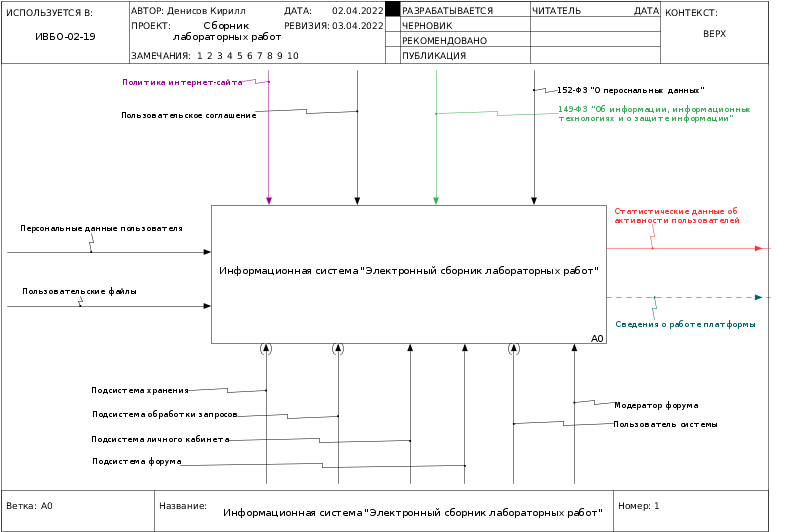
\includegraphics[width=0.8\linewidth]{images/ramus/01_A0}
	\caption{Контекстная диаграмма процесса предоставления услуг сервисом "Сборник лабораторных работ"}
	\label{fig:01a0}
\end{figure}



\end{document}

